\chapter{Introduction}\label{ch1}
\noindent
A real time system is any information processing system which has to respond to an externally generated input stimuli within 
a finite and specified period. Correctness of a real time system depends not only on the logical result of input but also on 
the time at which the result is produced. Different real time embedded systems include automobile systems, avionics systems 
and many others. Real time embedded systems which integrate tasks of different criticality levels on the same hardware 
platform are more commonly known as mixed criticality systems. In these systems, applications belonging to different 
criticality levels are engineered to different levels of assurance where high criticality applications are the 
costliest to design. Criticality level denotes the assurance against failure needed for a system component~\cite{burns2013mixed}.

\noindent
A task $\tau_{i}$ = $(A_{i}, D_{i}, C_{i}, E^{j}_{i})$ in a mixed criticality system is defined as 
follows:
\begin{itemize}
\item $A_{i} \in N$ denotes the arrival time,
% \newline
% \newline
% $P_{i} \in N$ denotes the period (time interval after which its next instance arrives),
% \newline
\item $D_{i} \in N$ and $D_{i} > A_{i}$ denotes the deadline,
\item $C_{i}$ denotes the set of criticality levels,
\item $E^{j}_{i} \in R$ denotes its execution time / memory budget at the $j^{th}$ criticality level.
\end{itemize}

\noindent
A mixed-criticality system (MCS) consists of tasks of two or more distinct levels of criticality. The main objective of 
mixed-criticality systems is to guarantee the safety of the system by increasing the number of execution of critical tasks. 
A mixed 
critical task has many execution modes and each mode is associated with different budgets for execution. Execution budget 
means resource requirement of a task in a particular execution mode. A task can switch from one mode to another mode 
if required. For example, a critical task generally executes in its lowest execution mode with minimum budget of execution in 
that mode. But it may switch to higher modes during execution with larger number of resources so that it may not miss its 
deadline. Scheduling critical tasks on a mixed criticality platform is quite challenging. We need to guarantee that all the 
critical tasks are to be scheduled and executed within their deadlines. 

\begin{figure}[t]
 \centering
 \fbox{
\includegraphics[width=13cm,height=10cm]{automobile_1.jpg}
}
\caption{Overview of an automotive system}
\label{fig3abc}
\end{figure}

\noindent
A popular example of a mixed criticality system is an automotive system.
Automotive embedded systems contain a mix of safety critical control tasks (needed for system stability and safety) and
time critical tasks with deadline constraints (needed for ensuring system performance and behavior). Safety critical
tasks include tasks for controlling vehicle dynamics, air-bag control which are crucial for ensuring the safety of the 
vehicle. On the other hand, tasks associated with stringent timing constraints like tasks for driver-assistance, help improve 
usability and driving comfort. Some tasks may also exhibit both timing and safety critical behavior. With the consolidation of 
functionality on the same hardware, applications with both classes of tasks may co-exist, interact and share common hardware 
platform resources like Electronic Control Units (ECUs), and buses. Scheduling and platform design to ensure such a mix of 
timing, control performance and stability constraints is a challenging problem. Fig\ref{fig3abc} gives an overview of an 
automotive system.


\noindent
In this type of mixed criticality systems, each task generally constitutes multiple instructions, some of which are compute 
intensive instructions, while others are memory intensive. Thus, memory intensive tasks require frequent memory accesses. But 
in our existing architecture, instructions cannot be served instantaneously as and when they arrive. A schematic diagram of a 
contemporary memory architecture is shown in Fig\ref{fig1ddd}. In existing computer architecture, we can schedule requests either 
at the processor or at the memory or more specifically the DRAM controller. Several scheduling algorithms have been proposed to 
schedule the tasks at the processor level. Uniprocessor schedulers mostly use Earliest Deadline First (EDF)~\cite{wiki:xxx2} 
or Rate Monotonic Scheduling (RMS)~\cite{wiki:xxx3} to schedule tasks at the processor. Scheduling of tasks in multi-core 
systems has also been proposed in~\cite{Giannopoulou:2013:SMA:2555754.2555771}. Current DRAM controllers take the advantage 
of row buffer locality. They follow an open row policy to schedule requests to access memory. According to the open row 
policy, the instruction which results in row hit is served first. Then the older requests are served in the order of their 
arrival. In this dissertation, we focus on the scheduling of memory requests at the DRAM so that maximum number of high 
critical tasks get executed.

\begin{figure}[t]
 
 \centering
 \fbox{
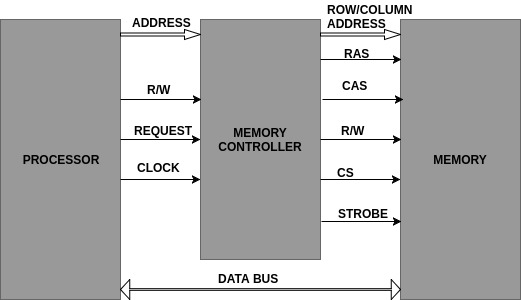
\includegraphics[width=10cm,height=7cm]{MEMORY.jpg}
}
\caption{Schematic diagram of memory architecture}
\label{fig1ddd}
\end{figure}

\section{Motivation of this dissertation}\label{motiv}
\noindent
In this dissertation, we study the problem of memory scheduling for mixed criticality systems. We first take up the problem of deciding the required number of banks that can ensure a given set of mixed criticality tasks can meet their deadlines. We study both the decision and optimization problems for the same. Following this, we take up the issue of bank scheduling. 
The major problem with the open row policy at the DRAM is that most of the high criticality tasks fail to meet their 
deadlines while waiting for memory access if not scheduled and executed within their deadlines.
Due to this open row policy, some low criticality tasks get prioritized to be executed first 
whereas, some high criticality tasks may miss their deadlines while waiting in the buffer for memory access. Thus, selection 
of tasks is a very important criteria for 
scheduling tasks of different criticality levels executing on such a platform in order to ensure safety of the system.
In this dissertation, we have proposed a novel method to schedule tasks around memory which increases the number of execution 
of high criticality tasks significantly. A number of proposals have been made for scheduling tasks of different criticality 
levels around memory. The fundamental difference of these methods with our proposed method is that in our proposed method, 
we ensure that no high criticality task will miss their deadlines at the cost of any low criticality task. This is the main 
motivation of this dissertation. The main contribution of this dissertation is highlighted below.

\section{Contribution of this dissertation}\label{contri}
\noindent
Our method proposes a bank aware memory scheduling policy to schedule tasks of different criticality levels across memory banks. 
We have partitioned the tasks across banks according to their address mapping and then we have refined our existing partitions 
by a heuristic partitioning algorithm which uses a cost function based on some task parameters and some system 
parameters as a metric for partitioning. Our proposed method has been compared with existing state-of-the-art memory 
controllers on different benchmarks of Malardalen Worst Case Execution Time Benchmark~\cite{gustafsson2010malardalen}. 
Results on different benchmarks show the efficiency of our proposed method. 
 

\section{Organization of this dissertation}\label{org}
\noindent
The rest of the dissertation is organized into 5 chapters. A summary of the contents of the chapters is as follows:
\begin{description}
 \item {\bf Chapter 2}: A detailed study of relevant research is presented here.
 
 \item {\bf Chapter 3}: This chapter deals with design specifications to support this type of mixed criticality system.
 
 \item {\bf Chapter 4}: This chapter addresses the inefficiency of existing DRAMs to support this type of mixed criticality
 system and our contribution to overcome this inefficiency.
 
 \item {\bf Chapter 5}: We summarise with conclusions on the contribution of our dissertation.
 
\end{description}

